\documentclass[12pt,graphicx,caption,rotating]{article}
\textheight=24cm
\textwidth=18cm
\topmargin=-2cm
\oddsidemargin=0cm
\usepackage[utf8x]{inputenc}
\usepackage[activeacute,spanish]{babel}
\usepackage{amssymb,amsfonts}
\usepackage[tbtags]{amsmath}
\usepackage{pict2e}
\usepackage{float}
\usepackage[all]{xy}
\usepackage{graphics,graphicx,color,colortbl}
\usepackage{times}
\usepackage{subfigure}
\usepackage{wrapfig}
\usepackage{multicol}
\usepackage{cite}
\usepackage{url}
\usepackage[tbtags]{amsmath}
\usepackage{amsmath,amssymb,amsfonts,amsbsy}
\usepackage{bm}
\usepackage{algorithm}
\usepackage{algorithmic}
\usepackage[centerlast, small]{caption}
\usepackage[colorlinks=true, citecolor=blue, linkcolor=blue, urlcolor=blue, breaklinks=true]{hyperref}
\hyphenation{ele-men-tos he-rra-mi-en-ta cons-tru-yen trans-fe-ren-ci-a pro-pu-es-tas si-mu-lar vi-sua-li-za-cion}

\begin{document}
\title{\textbf{\huge{Primer Parcial de Microondas - Caracterización de elementos.}}}
\author{David Ricardo Martínez Hernández \textbf{Código:} 261931\\
	\href{}{drmartinezhe@unal.edu.co}\\
	Universidad Nacional de Colombia}
\date{}
\maketitle

\section{Introducción}
\noindent
Las ondas electromagnéticas tienen la propiedad de propagarse en forma de voltaje o corriente por un medio guiado o en el espacio libre como onda electromagnética. Su estudio y comprensión se manifiesta bajo la solución en forma de onda que se pueden obtener de las ecuaciones de Maxwell. La característica esencial de este tipo de ondas es que no necesitan de un medio en especial para propagarse, esto quiere decir que lo pueden hacer en el vacío.\\
El espectro electromagnético se extiende desde las bajas frecuencias usadas para la radio moderna (extremo de la onda larga) hasta los rayos gamma (extremo de la onda corta), que cubren longitudes de onda de entre miles de kilómetros y la fracción del tamaño de un átomo.

\section{Cable $NMS−RG142−40.0−NMS$}
\noindent
Características:
\begin{itemize}
 \item Rendimiento de hasta 18 GHz.
 \item Asambleas flexibles rentables.
 \item Variedad de construcción para aplicaciones que requieren:
 \begin{itemize}
  \item Mayor flexibilidad.
  \item Mejora de Blindaje.
  \item Baja pérdida de inserción.
 \end{itemize}
\end{itemize}
\noindent
Aplicaciones típicas:
\begin{itemize}
 \item Componente Interconexiones.
 \item Cables de prueba.
 \item Asambleas de puente.
 \item Asambleas In − Box.
\end{itemize}
\noindent
Conectores disponibles:
Esta familia de cables ofrece una amplia variedad de conectores. Las interfaces disponibles serán dictadas en gran medida por el diámetro del cable seleccionado . Las interfaces habituales son: \textbf{SMA, SSMA, MCX, MMCX} y \textbf{SMB} para los cables de menor diámetro y \textbf{tipo N, TNC} y \textbf{BNC} para los cables de mayor diámetro.\\
El Cuadro \ref{tab1} muestra algunas características del cable $NMS−RG142−40.0−NMS$:

\begin{table}[H]
  \centering
  \caption{Aspectos Técnicos cable RG142 \cite{page1}.}
  \begin{tabular}{|c|c|} \hline
    \multicolumn{ 1}{|c|}{} & NEC CMP rated. Dual silver shields. Brown tinted \\ 
    \multicolumn{ 1}{|c|}{Resumen} & FEP jacked. Passes VW1 Vertical Wire Test. If Mil \\ 
    \multicolumn{ 1}{|c|}{} & Spec MIL-C-17G rated; it may not be available in \\ 
    \multicolumn{ 1}{|c|}{} & long continuous runs. Losses per $100$. \\ \hline
    Tipo de cable & $3/16”$ \\ \hline
    Tipo de bobina & D \\ \hline
    Aislamiento & Extruido de doble escudo PTFE \\ \hline
    Ctr Cond & $0.037$ Soild \\ \hline
    Nominal Core O.D. & $0.116$ \\ \hline
    Nominal O.D. & $0.195$ \\ \hline
    VOP & $70,9\,\%$ \\ \hline
    Shield \% & $98\,\%$ \\ \hline
    Capacitancia nominal (Pf/ft) & $32$ \\ \hline
    Perdidas $@ 100\,MHz$ & $5,5\, dB$ \\ \hline
    Perdidas $@ 400\,MHz$ & $11,7\, dB$ \\ \hline
    Perdidas $@ 1000\,MHz$ & $19,0\, dB$ \\ \hline
    Otros Aspectos & Mil Spec $MIL-C-17G$ \\ \hline
    Impedancia & $50\, \Omega$ \\ \hline
    Garantía & $1$ Año \\ \hline
  \end{tabular}
  \label{tab1}
\end{table}
\noindent
La lectura correcta de este cable es la mostrada en la Figura~\ref{fig1}
\begin{figure}[H]
	\centering
		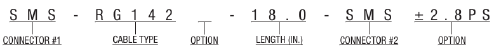
\includegraphics[scale=0.5]{fig1.png}
	\caption{Forma correcta de realizar la lectura de la referencia del cable \cite{page3}.}
	\label{fig1}
\end{figure}

\subsection{}
\noindent
La Figura~\ref{fig2} representa los datos obtenidos por el analizador para los cables:
\begin{figure}[H]
  \centering
  \begin{minipage}{8cm}
    \begin{subfigure}
      [Datos obtenidos del Analizador de espectros para el cable N~1.]{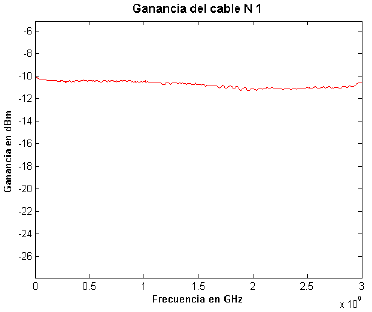
\includegraphics[scale=0.6] {fig2.png}\label{fig2}}
    \end{subfigure}
  \end{minipage}
  \begin{minipage}{8cm}
    \begin{subfigure}
      [Datos obtenidos del Analizador de espectros para el cable N~2.]{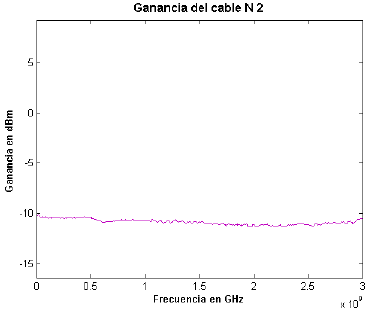
\includegraphics[scale=0.6] {fig3.png}\label{fig3}}
    \end{subfigure}
  \end{minipage}
  \begin{subfigure}
    [Datos obtenidos del Analizador de espectros para el cable N~3.]{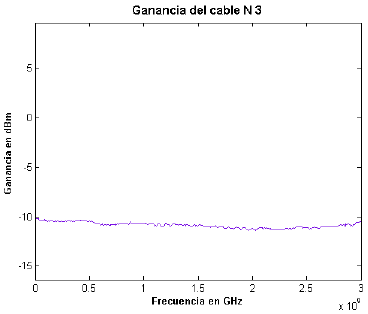
\includegraphics[scale=0.6] {fig4.png}\label{fig4}}
  \end{subfigure}
  \caption{Datos obtenidos del Analizador de espectros.}
  \label{fig01}
\end{figure}
\noindent
Al comparar los valores obtenidos en las Figuras~\ref{fig2},~\ref{fig3}~y~\ref{fig4} con los valores del Cuadro~\ref{tab2} se puede concluir que las perdidas de los cables en el rango de los $0\, M Hz$ a los $3\, GHz$ los cables tienen un comportamiento muy similar, las caracterizaciones fueron tomados con los mismos valores (ver Cuadro~\ref{tab2}).
\begin{table}[H]
  \centering
  \caption{Especificaciones de la toma de medidas.}
    \begin{tabular}{|c|c|c|c|c|c|}\hline
      \textbf{Cable } & \textbf{Longitud (m) } & \textbf{RBW (KHz) } & \textbf{SWP (s) } & \textbf{Span (GHz) } & \textbf{Center (GHz) } \\ \hline
      \textbf{1} & $0,98$  & \multicolumn{ 1}{c|}{} & \multicolumn{ 1}{c|}{} & \multicolumn{ 1}{c|}{} & \multicolumn{ 1}{c|}{} \\ \cline{ 1- 2}
      \textbf{2} & $0,97 $ & \multicolumn{ 1}{c|}{$10$} & \multicolumn{ 1}{c|}{$75$} & \multicolumn{ 1}{c|}{$3$} & \multicolumn{ 1}{c|}{$1,5 $} \\ \cline{ 1- 2}
      \textbf{3} & $0,97$ & \multicolumn{ 1}{c|}{} & \multicolumn{ 1}{c|}{} & \multicolumn{ 1}{c|}{} & \multicolumn{ 1}{c|}{} \\ \hline
    \end{tabular}
  \label{tab2}
\end{table}

\section{Cable $RF\, L1803$ y $RF\, L1807$}
\noindent
El cable N 4 se encuentra fallando se tomaron los datos del cable funcionando adecuadamente y fallando
(ver Figuras~\ref{fig5}~y~\ref{fig6}).
\begin{figure}[H]
  \centering
  \begin{minipage}{8cm}
    \begin{subfigure}
      [Datos obtenidos del Analizador de espectros para el cable funcionando.]{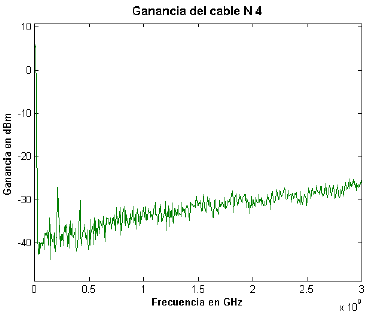
\includegraphics[scale=0.6] {fig5.png}\label{fig5}}
    \end{subfigure}
  \end{minipage}
  \begin{minipage}{8cm}
    \begin{subfigure}
      [Datos obtenidos del Analizador de espectros para el cable fallando.]{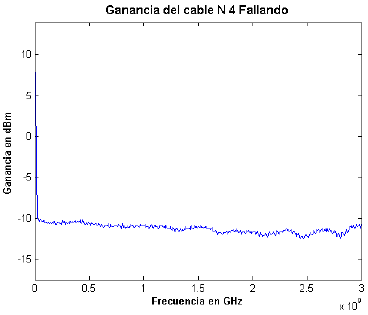
\includegraphics[scale=0.6] {fig6.png}\label{fig6}}
    \end{subfigure}
  \end{minipage}
  \caption{Datos obtenidos del Analizador de espectros.}
  \label{fig02}
\end{figure}
\noindent
\textbf{Nota:} Falla alguna de las conexiones que van al analizador, se tomo imagen de falla e imagen estable. A demás tiene un certificado de vencimiento del año 2010, y esta calibrado en el año $2009$.\\\\
El cable N 5 de referencia $RF\, L1807$ en la Figura \ref{fig7} se encuentra la gráfica de salida.
\begin{figure}[H]
	\centering
		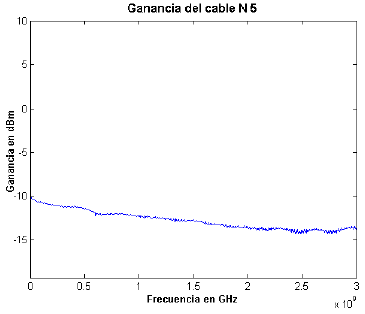
\includegraphics[scale=0.6]{fig7.png}
	\caption{Datos obtenidos del Analizador de espectros para el cable N~5.}
	\label{fig7}
\end{figure}
\noindent
Para esta serie de cables no se encontró información alguna, por eso no se pudo realizar un análisis con los cables de fabrica.\\
Los medidas que se utilizaron en el analizador son (ver Cuadro \ref{tab3}):
\begin{table}[H]
  \centering
  \caption{Especificaciones de la toma de medidas.}
  \begin{tabular}{|c|c|c|c|c|c|}\hline
    \textbf{Cable } & \textbf{Longitud (m) } & \textbf{RBW (KHz) } & \textbf{SWP (s) } & \textbf{Span (GHz) } & \textbf{Center (GHz) } \\ \hline
    \textbf{4} & $2,95 $ & \multicolumn{ 1}{c|}{$10$} & \multicolumn{ 1}{c|}{$75$} & \multicolumn{ 1}{c|}{$3$} & \multicolumn{ 1}{c|}{$1,5 $} \\ \cline{ 1- 2}
    \textbf{5} & $0,6,97$ & \multicolumn{ 1}{c|}{} & \multicolumn{ 1}{c|}{} & \multicolumn{ 1}{c|}{} & \multicolumn{ 1}{c|}{} \\ \hline
  \end{tabular}
    \label{tab3}
\end{table}

\section{Cable 6: $ST18/SMAm/SMAm/72$}
\noindent
Los resultados obtenidos de la caracterización se encuentra en la Figura~\ref{fig8}.
\begin{figure}[H]
	\centering
		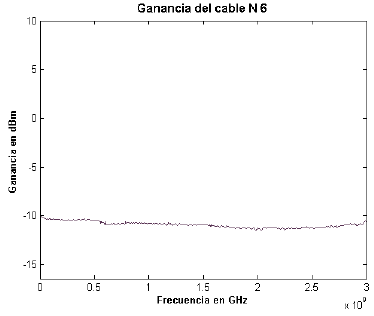
\includegraphics[scale=0.6]{fig8.png}
	\caption{Datos obtenidos del Analizador de espectros para el cable N~6.}
	\label{fig8}
\end{figure}
\noindent
Los medidas que se utilizaron en el analizador son (ver Cuadro~\ref{tab4}):
\begin{table}[H]
  \centering
  \caption{Especificaciones de la toma de medidas.}
    \begin{tabular}{|c|c|c|c|c|c|}\hline
      \textbf{Cable } & \textbf{Longitud (m) } & \textbf{RBW (KHz) } & \textbf{SWP (s) } & \textbf{Span (GHz) } & \textbf{Center (GHz) } \\ \hline
      \textbf{6} & $1,75$  & $10$ & $75$ & $3$ & $1,5$  \\ \hline
    \end{tabular}
  \label{tab4}
\end{table}
\noindent
Los datos de operación que da el fabricante se encuentran en \cite{page3}, al comparar los datos obtenidos gráficamente con los suministrados por el fabricante se puede determinar que el cable se encuentra en buen estado.

\section{Cable 7 y Cable 8}
\begin{figure}[H]
  \centering
  \begin{minipage}{8cm}
    \begin{subfigure}
      [Datos obtenidos del Analizador de espectros para el cable N~7.]{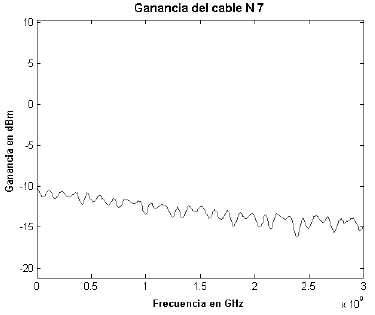
\includegraphics[scale=0.6] {fig9.png}\label{fig9}}
    \end{subfigure}
  \end{minipage}
  \begin{minipage}{8cm}
    \begin{subfigure}
      [Datos obtenidos del Analizador de espectros para el cable N~8.]{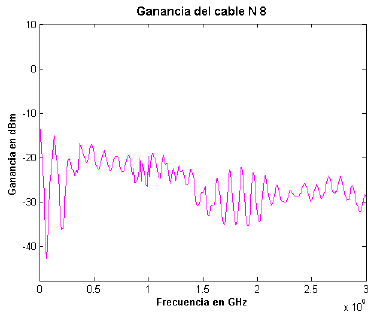
\includegraphics[scale=0.6] {fig10.png}\label{fig10}}
    \end{subfigure}
  \end{minipage}
  \caption{Datos obtenidos del Analizador de espectros.}
  \label{fig02}
\end{figure}
\noindent
Para el cable N~7 se realizo conexión VNC en ambos extremos y se hizo adaptación a tipo N.\\
Para el cable N~8 se realizo arreglo de caimanes con conexión VNC en ambos extremos, adaptación a tipo~N en ambos extremos.\\\\
Como se puede observar en las Figuras \ref{fig9} y \ref{fig10} son los peores cables que se pueden utilizar al realizar pruebas en alta frecuencia, tienen un comportamiento muy decreciente, es decir sus valores tienden a cero, se vuelven grandes atenuadores a altas frecuencias.\\
Los medidas que se utilizaron en el analizador son (ver Cuadro~\ref{tab5}):
\begin{table}[H]
  \centering
  \caption{Especificaciones de la toma de medidas.}
  \begin{tabular}{|c|c|c|c|c|c|}\hline
    \textbf{Cable } & \textbf{Longitud (m) } & \textbf{RBW (KHz) } & \textbf{SWP (s) } & \textbf{Span (GHz) } & \textbf{Center (GHz) } \\ \hline
    \textbf{7} & $0,97 $ & \multicolumn{ 1}{c|}{$10$} & \multicolumn{ 1}{c|}{$75$} & \multicolumn{ 1}{c|}{$3$} & \multicolumn{ 1}{c|}{$1,5 $} \\ \cline{ 1- 2}
    \textbf{8} & $2$ & \multicolumn{ 1}{c|}{} & \multicolumn{ 1}{c|}{} & \multicolumn{ 1}{c|}{} & \multicolumn{ 1}{c|}{} \\ \hline
  \end{tabular}
    \label{tab5}
\end{table}

\section{Caracterización del Bridge}
\noindent
Para poder determinar la ganancia de la antena y del atenuador es necesario caracterizar el Bridge.
\begin{figure}[H]
  \centering
  \begin{minipage}{8cm}
    \begin{subfigure}
      [Transmisión de entrada a salida.]{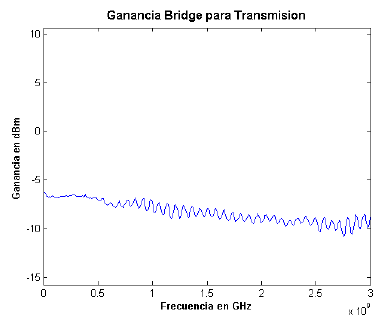
\includegraphics[scale=0.6] {fig11.png}\label{fig11}}
    \end{subfigure}
  \end{minipage}
  \begin{minipage}{8cm}
    \begin{subfigure}
      [Transmisión de entrada a reflexión.]{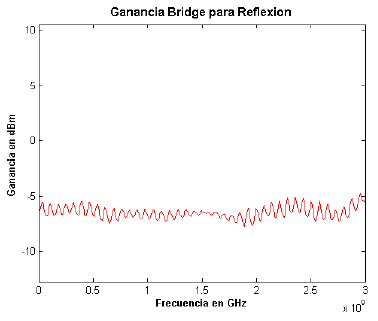
\includegraphics[scale=0.6] {fig12.png}\label{fig12}}
    \end{subfigure}
  \end{minipage}
  \caption{Datos obtenidos del Analizador de espectros.}
  \label{fig03}
\end{figure}
\noindent
Los valores utilizados en el analizador fueron (ver Cuadro~\ref{tab6})
\begin{table}[H]
  \centering
  \caption{Transmisión de entrada a salida.}
    \begin{tabular}{|c|c|c|c|c|}\hline
      \textbf{Acción } & \textbf{RBW (KHz) } & \textbf{SWP (s) } & \textbf{Span (GHz) } & \textbf{Center (GHz) } \\ \hline
      \textbf{Transmisión } & \multicolumn{ 1}{c|}{10} & \multicolumn{ 1}{c|}{75} & \multicolumn{ 1}{c|}{3} & \multicolumn{ 1}{c|}{1,5 } \\ \cline{ 1- 1}
      \textbf{Reflexión} & \multicolumn{ 1}{c|}{} & \multicolumn{ 1}{c|}{} & \multicolumn{ 1}{c|}{} & \multicolumn{ 1}{c|}{} \\ \hline
    \end{tabular}
  \label{tab6}
\end{table}

\begin{table}[H]
  \centering
  \caption{Transmisión de entrada a salida.}
    \begin{tabular}{|c|c|}\hline
      \textbf{Frecuencia (GHz) } & \textbf{Atenuación (dBm) } \\ \hline
      $1704$ & $−8,94 $ \\ \hline
      $2,4 $ & $−8,66 $ \\ \hline
    \end{tabular}
  \label{tab7}
\end{table}

\begin{table}[H]
  \centering
  \caption{Transmisión de entrada a reflexión.}
    \begin{tabular}{|c|c|}\hline
      \textbf{Frecuencia (GHz) } & \textbf{Atenuación (dBm) } \\ \hline
      $1704$ & $−6,63 $ \\ \hline
      $2,4 $ & $−6.25 $ \\ \hline
    \end{tabular}
  \label{tab8}
\end{table}

\section{Bridge y resistencias}

\begin{figure}[H]
  \centering
  \begin{minipage}{8cm}
    \begin{subfigure}
      [Transmisión de entrada con $R = \infty$.]{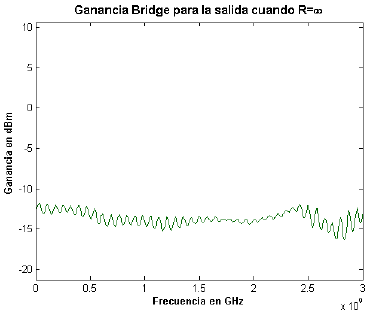
\includegraphics[scale=0.6] {fig13.png}\label{fig13}}
    \end{subfigure}
  \end{minipage}
  \begin{minipage}{8cm}
    \begin{subfigure}
      [Transmisión de entrada con $R = 50 \Omega$.]{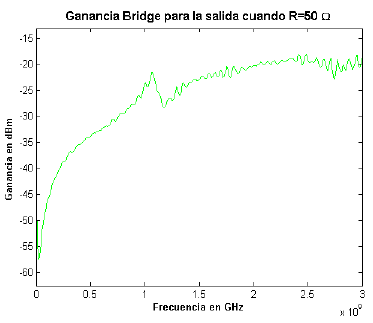
\includegraphics[scale=0.6] {fig14.png}\label{fig14}}
    \end{subfigure}
  \end{minipage}
  \begin{subfigure}
    [Transmisión de entrada con resistencia de potencia.]{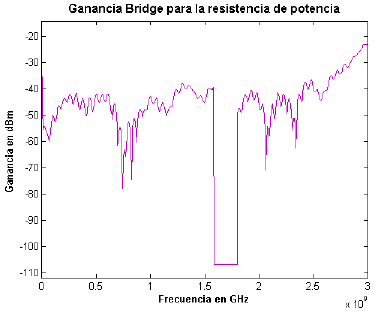
\includegraphics[scale=0.7] {fig15.png}\label{fig15}}
  \end{subfigure}
  \caption{Datos obtenidos del Analizador de espectros.}
  \label{fig04}
\end{figure}

\begin{table}[H]
  \centering
  \caption{Transmisión de entrada con $R = \infty$.}
    \begin{tabular}{|c|c|}\hline
      \textbf{Frecuencia (GHz) } & \textbf{Atenuación (dBm) } \\ \hline
      $1704$ & $−13,75 $ \\ \hline
      $2,4 $ & $−12.5 $ \\ \hline
    \end{tabular}
  \label{tab9}
\end{table}

\begin{table}[H]
  \centering
  \caption{Transmisión de entrada con $R = 50 \Omega$.}
    \begin{tabular}{|c|c|}\hline
      \textbf{Frecuencia (GHz) } & \textbf{Atenuación (dBm) } \\ \hline
      $1704$ & $−6,63 $ \\ \hline
      $2,4 $ & $−6.25 $ \\ \hline
    \end{tabular}
  \label{tab10}
\end{table}
\noindent
Para la resistencia de potencia los valores obtenidos a los $1,7\, GHz$ tiene una ganancia que tiende a cero, es decir es un filtro a esa frecuencia, y a los $2,4\, GHz$ no se tomaron datos. A demás se utilizaron los cables N~2, N~3 y N~6 con el puente de retorno.

\section{Atenuador y Antena}
\noindent
El atenuador es de referencia $LF P − 50$ de $20\, dB$ y la antena es de referencia $Guia\,de\, 3,40$.
\begin{figure}[H]
  \centering
  \begin{minipage}{8cm}
    \begin{subfigure}
      [Transmisión de entrada a atenuador.]{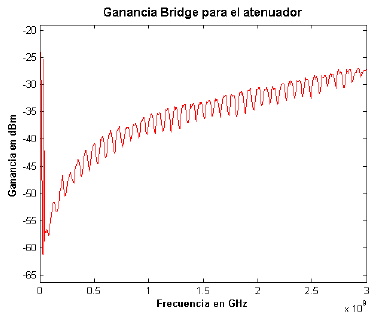
\includegraphics[scale=0.6] {fig16.png}\label{fig16}}
    \end{subfigure}
  \end{minipage}
  \begin{minipage}{8cm}
    \begin{subfigure}
      [Transmisión de entrada a excitador y antena.]{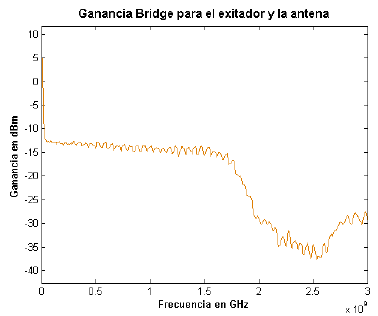
\includegraphics[scale=0.6] {fig17.png}\label{fig17}}
    \end{subfigure}
  \end{minipage}
  \caption{Datos obtenidos del Analizador de espectros.}
  \label{fig03}
\end{figure}
\noindent
Para el atenuador se utilizo el cable N 2 y se obtuvieron los siguientes resultados (ver Cuadro \ref{tab11})
\begin{table}[H]
  \centering
  \caption{Transmisión con el atenuador.}
    \begin{tabular}{|c|c|}\hline
      \textbf{Frecuencia (GHz) } & \textbf{Atenuación (dBm) } \\ \hline
      $1704$ & $−31.86$ \\ \hline
      $2,4 $ & $−31.19$ \\ \hline
    \end{tabular}
  \label{tab11}
\end{table}

\begin{table}[H]
  \centering
  \caption{Transmisión con la antena.}
    \begin{tabular}{|c|c|}\hline
      \textbf{Frecuencia (GHz) } & \textbf{Atenuación (dBm) } \\ \hline
      $1704$ & $−15.4$ \\ \hline
      $2,4 $ & $−36$ \\ \hline
    \end{tabular}
  \label{tab12}
\end{table}
\noindent
Al utilizar la antena se midieron las reflexiones, utilizando el cable N~2, N~3 y N~6,con el puente de perdidas.

\section{Conclusiones}

\begin{itemize}
 \item Al utilizar los cables con terminación en caimán se pudo observar que tienen un mal comportamiento en altas frecuencias, esto puede deberse a los cables utilizados los cuales no tenían referencia alguna, a demás los caimanes no son buenos transmisores ni receptores.
 \item Los cables N 1, N 2, N 3, N 5 y N 6 son muy buenos, tienen un comportamiento muy similar tanto en altas frecuencias como en bajas. Comparados con los cables N 4, N 7 y N 8 atenúan mucho la señal, esto hace que tengan muchas perdidas y la señal se pierde.
 \item Todas las medidas del Brigdge y demás elementos que se utilizaron con el se tomaron con los mismos valores del Cuadro~\ref{tab6}, esto facilito la caracterizaciones de los elementos.
\end{itemize}

\begin{thebibliography}{99}
 
 \bibitem{pozar} Pozar, David M.
 {\em "`Microwave engineering"'}.
 Jhon Wiley \& Son, Inc., Fourth Edition, 2012.

 \bibitem{page1} Tessco Reference Manual [en línea]. Disponible en \url{http://www.tessco.com/productsdisplayProductInfo.do?sku=86717&eventPage=1} [consultado 8 noviembre 2013].
 
 \bibitem{page2} RFMW Reference Manual [en línea]. Disponible en \url{http://www.rfmw.com/dataFLRF-CABLE-CATALOG.pdf} [consultado 8 noviembre 2013].
 
 \bibitem{page3}RFMD Reference Manual [en línea]. Disponible en \url{http://download.siliconexpertcom/pdfs/2007/06/22/c/cs/hps/ds/st-18.s.pdf} [consultado 8 noviembre 2013].
 
\end{thebibliography}
\end{document}